% !TEX root = ../Tesis_NataliaOpazo.tex 

A continuación se presentan los efectos generados por la inserción de los campos de flujo de polvo en los niveles de pCO$_2$ atmosférico según el modelo cGENIE, entre el periodo del Holoceno hasta el UMG. 

\section{Resultados globales}

En la figura \ref{fig:All}, la trayectoria del nivel de pCO$_2$ en todas las simulaciones pueden ser explicada por una función logaritmo. Sin embargo, Takemura muestra una pequeña desviación en el nivel 7 (con aproximadamente 9.5 ppm de reducción). Sin embargo, lo anterior no se condice con el aumento progresivo de polvo desde el Holoceno hasta el UMG para este caso. 

La simulación Albani es la que muestra mayor reducción de pCO$_2$ ($\sim 21$ ppm.). Seguido por el modelo MIROC-ESM ($\sim 20$ ppm). La máxima captación de Albani, puede ser producto de la diferencia intermedia de polvo entre el periodo del Holoceno y del UMG en comparación a los otros casos. Albani además, posee los niveles más altos de depositación de polvo durante el periodo del Holoceno (aunque es el tercer flujo de polvo durante el UMG). Esto habría dado un importante input inicial al modelo cGENIE que se mantuvo con valores altos hacia el final de la simulación (UMG). \newpage

\begin{figure}[H]
        \begin{subfigure}[b]{0.5\textwidth}
                \includegraphics[width=\linewidth]{../../Figuras/Globales/Albani/All}
                \caption{Albani}
                \label{fig:A_All}
        \end{subfigure}%
                \begin{subfigure}[b]{0.5\textwidth}
                \includegraphics[width=\linewidth]{../../Figuras/Globales/Lambert/All}
                \caption{Lambert}
                \label{fig:L_All}
        \end{subfigure}%

        \begin{subfigure}[b]{0.5\textwidth}
                \includegraphics[width=\linewidth]{../../Figuras/Globales/Takemura/All}
                \caption{Takemura}
                \label{fig:T-All}
        \end{subfigure}%
        \begin{subfigure}[b]{0.5\textwidth}
                \includegraphics[width=\linewidth]{../../Figuras/Globales/MIROC-ESM/All}
                \caption{MIROC-ESM}
                \label{fig:MI-All}
        \end{subfigure}
        
        \begin{subfigure}[b]{0.5\textwidth}
                \includegraphics[width=\linewidth]{../../Figuras/Globales/MRI-CGCM3/All}
                \caption{MRI-CGCM3}
                \label{fig:MR-All}
        \end{subfigure}
        \caption[Series de reducci\'on de $pCO_2$ de flujos globales de polvo]{Series de reducci\'on de $pCO_2$ obtenidos mediante simulaci\'on cGENIE, desde el Holoceno hasta el \'Ultimo M\'aximo Glacial para flujos de polvo globales.}\label{fig:All}
\end{figure}

 La simulación Lambert es la que presenta mayor diferencia entre el nivel de polvo del Holoceno y el UMG. Este tiene lo más elevados flujos de polvo para el UMG, dando una reducción de $\sim 16.5$ ppm. La simulación Lambert tiene el tercer valor más alto de disminución de pCO$_2$ atmosférico, seguido por el modelo Takemura ($\sim 16$ ppm.). Este último tiene los mayores flujos de polvo en el Holoceno pero capturas más bajas que Lambert hacia el UMG. La simulación MRI-CGCM3 posee los menores flujos de polvo y presenta la menor disminución de pCO$_2$, estimada en aproximadamente 9 ppm. \newpage

\section{Resultados regionales}
A continuaci\'on se presentan los resultados correspondiente a cada zona HNLC que se muestra en la figura \ref{fig:Grilla4}.

\subsection{Pac\'ifico Norte}

\begin{figure}[H]
\centering
 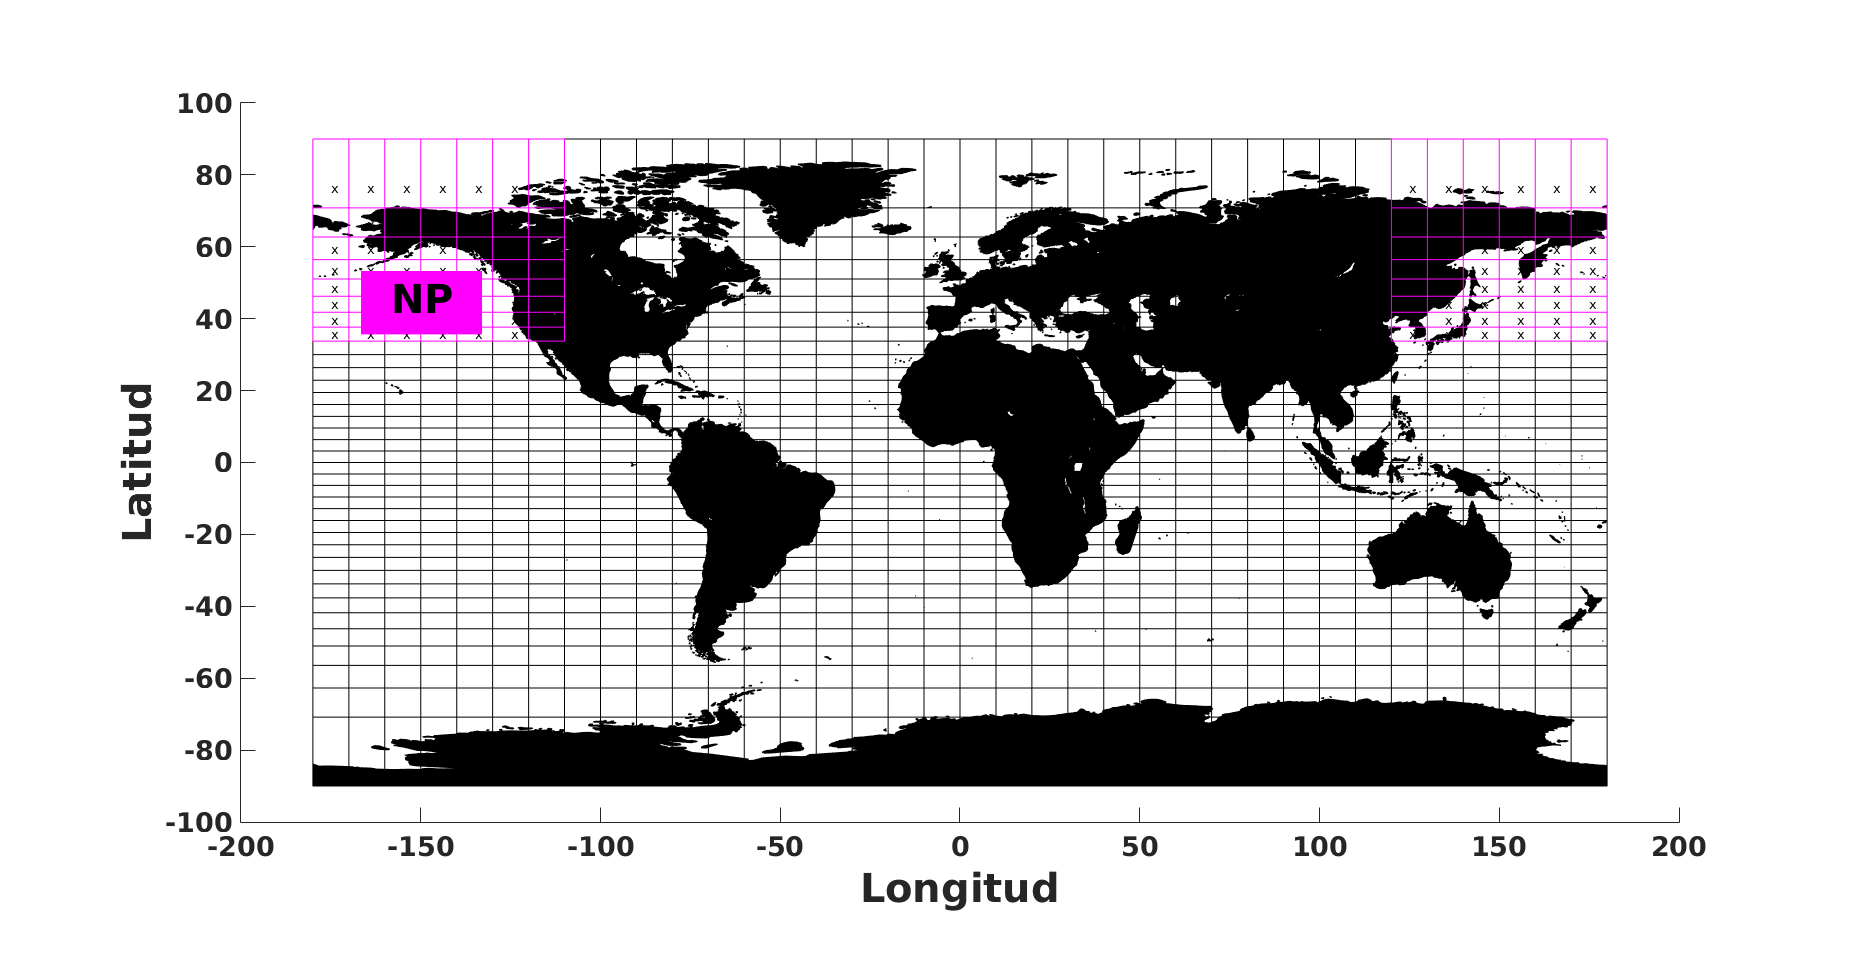
\includegraphics[width=0.8\textwidth]{mapa3_2_NP.png}
 \caption[Figura región del Pacífico Norte]{Mapa global, que muestra la región del Pacífico Norte que fue aislada en la simulación cGENIE.}
  \label{fig:Mapa_NP}
\end{figure}

\begin{table}[H]
\centering
\begin{tabular}{|c|c|c|c|c|}
\hline
& \multicolumn{4}{c|}{Reducci\'on de $pCO_2$ global} \\
\cline{2-5}
Modelo& Ajuste & Par\'ametros & R-cuadrado ($R^2$) & RMSE\\
\hline \hline
Lambert  & Logar\'itmico  & p1=-29.66, p2=5805 y p3=3.495 & 0.9975 & 0.0945 \\ \hline
Albani & Logar\'itmico & p1=-18.23, p2=-2382 y p3=-2382 & 0.9995 & 0.0613\\ \hline
Takemura & Logar\'itmico & p1=-16.09, p2=291 y p3=2.524 & 0.9999 & 0.0034\\ \hline
MIROC-ESM & Logar\'itmico & p1=-50.18, p2=3916 y p3=6.65 & 0.9984 & 0.0863
\\ \hline
MRI-CGCM3 & Logar\'itmico & p1=-39.01, p2=-126.5 y p3=5.074 & 0.9998 & 0.0132\\ \hline
\end{tabular}
\caption[Coeficientes del ajuste NP]{Caracter\'isticas de los ajustes realizados a las reducciones globales de $pCO_2$, a partir de los resultados del modelo cGENIE. El ajuste general es logar\'itmico, 
su ecuaci\'on est\'andar es: $ f(x)=p1 + \frac{p2}{x} + p3*log(x)$. Donde f(x) es la reducci\'on de $pCO_2$ y x, el flujo de polvo de cada nivel para la zona del Pacífico Norte. } 
\label{tabla:NP}
\end{table} \newpage

 \begin{figure}[H]
        \begin{subfigure}[b]{0.5\textwidth}
                \includegraphics[width=\linewidth]{../../Figuras/Regionales/Albani/NP}
                \caption{Albani}
                \label{fig:A_R_NP}
        \end{subfigure}%
                \begin{subfigure}[b]{0.5\textwidth}
                \includegraphics[width=\linewidth]{../../Figuras/Regionales/Lambert/NP}
                \caption{Lambert}
                \label{fig:L_R_NP}
        \end{subfigure}%
        
        \begin{subfigure}[b]{0.5\textwidth}
                \includegraphics[width=\linewidth]{../../Figuras/Regionales/Takemura/NP}
                \caption{Takemura}
                \label{fig:T_R_NP}
        \end{subfigure}%
        \begin{subfigure}[b]{0.5\textwidth}
                \includegraphics[width=\linewidth]{../../Figuras/Regionales/MIROC-ESM/NP}
                \caption{MIROC-ESM}
                \label{fig:MI_R_NP}
        \end{subfigure}
        
        \begin{subfigure}[b]{0.5\textwidth}
                \includegraphics[width=\linewidth]{../../Figuras/Regionales/MRI-CGCM3/NP}
                \caption{MRI-CGCM3}
                \label{fig:MR_R_NP}
        \end{subfigure}
        \caption[Series de reducci\'on de $pCO_2$ de flujos regionales de polvo (NP)]{Reducci\'on de $pCO_2$ obtenidos mediante simulaci\'on cGENIE, para flujos de polvo cambiantes en la zona del Pacífico Norte (NP) desde el Holoceno hasta el \'Ultimo M\'aximo Glacial.}\label{fig:NP}
\end{figure}

La mayor reducción de pCO$_2$ en esta zona fue estimada por la simulación Albani ($\sim 7$ ppm durante el UMG).
La razón positiva de polvo durante la terminación I ($\sim 0.5$, ver anexos \ref{fig:A}), y las distribuciones de polvo presentes en Albani (figura \ref{fig:Albani}), nos evidencian un gran flujo en el Pacífico Norte. No obstante, este flujo de polvo no es superior a los flujos presentes en Lambert, que producen una captura de pCO$_2$ alrededor de 5 ppm en el UMG. Éste valor, es ligeramente inferior a lo estimado para el modelo MIROC-ESM ($\sim 5.53$ ppm). De esta manera, si bien los flujos de polvo son mayores para el caso de Lambert, es su propia variabilidad la que produciría una menor captura de pCO$_2$ atmosférico por parte de los océanos en esta región. Mientras que, por otro lado, MIROC-ESM tiene flujos excesivamente inferiores, pero posee una tasa de depositación mayor en el área de interés (ver Anexos figura \ref{fig:MI} y \ref{fig:MIROC}). 

La simulación MRI-CGCM3 tiene una disminución de pCO$_2$ menor que los modelos previamente mencionados ($\sim 2.5$ p.p.m.), aunque tenuemente superior a Takemura ($\sim 1.14$ p.p.m.). Takemura es el caso con los más bajos flujos de polvo en la región. Los Flujos de polvo MRI-CGCM3 son similares a los de MIROC-ESM en la zona (ver Anexos \ref{fig:MI} y \ref{fig:MR}). De esta manera su diferencia se atribuye, por un lado, a una constante mayor tasa de depositación de polvo en la región (ver figuras \ref{fig:MRI} y \ref{fig:MIROC}), y por otro, a un input inicial (condición de campo de polvo global Holoceno) sustancialmente diferente a MIROC-ESM. 


\subsection{Pac\'ifico Central}

\begin{figure}[H]
\centering
 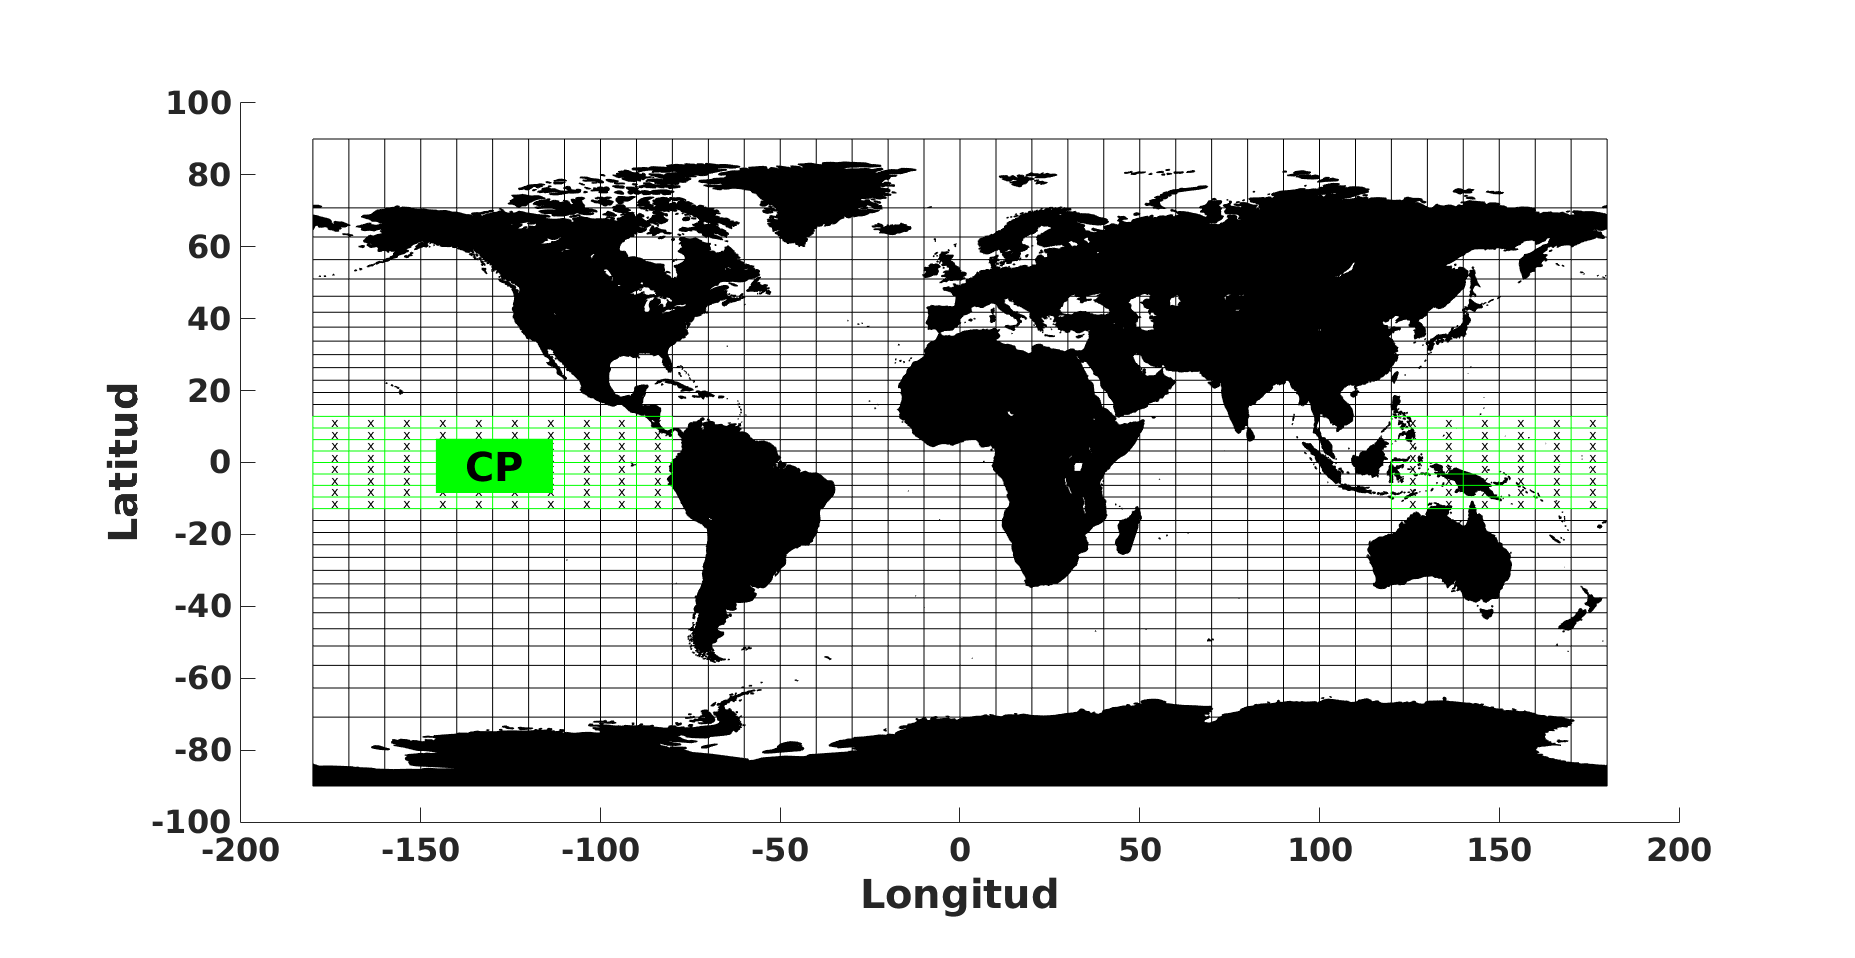
\includegraphics[width=0.8\textwidth]{mapa3_2_CP.png}
 \caption[Figura región del Pacífico Central]{Mapa global, que muestra la región del Pacífico Central que fue aislada en la simulación cGENIE.}
  \label{fig:Mapa_CP}
\end{figure}
\newpage

\begin{table}[H]
\centering
\begin{tabular}{|c|c|c|c|c|}
\hline
& \multicolumn{4}{c|}{Reducci\'on de $pCO_2$ global} \\
\cline{2-5}
Modelo& Ajuste & Par\'ametros & R-cuadrado ($R^2$) & RMSE\\
\hline \hline
Lambert  & Logar\'itmico  & p1=-22.48, p2=533.5 y p3=3.261 & 1 & 0.0029 \\ \hline
%Albani & Logar\'itmico & p1=2.1 y p2=2.20$e^{-7}$& 0.998 & 0.06854\\ \hline
Takemura & Logar\'itmico & p1=-26.89, p2=631.4 y p3=4.256 & 0.9997 & 0.0165\\ \hline
MIROC-ESM & Logar\'itmico & p1=-33.13, p2=1011 y p3=5.237 & 0.9986 & 0.0518\\ \hline
MRI-CGCM3 & Logar\'itmico & p1=-15.38, p2=180.5 y p3=2.74 & 0.9999 & 0.0028\\ \hline
\end{tabular}
\caption[Coeficientes de ajuste CP]{Caracter\'isticas de los ajustes realizados a las reducciones globales de $pCO_2$, a partir de los resultados del modelo cGENIE. El ajuste general es logar\'itmico, 
su ecuaci\'on est\'andar es: $ f(x)=p1 + \frac{p2}{x} + p3*log(x)$. Donde f(x) es la reducci\'on de $pCO_2$ y x, el flujo de polvo de cada nivel para la zona del Pacífico central.}
\label{tabla:Res3}
\end{table}

Los valores de reducción de pCO$_2$ en esta zona son en general bajos y similares. El comportamiento de la simulación es descrita por una función logarítmica. La corta distancia entre los campos de polvo del Holoceno y UMG en cada una de los casos hacen que esta reducción sea similar a una función lineal.  

El mayor aporte es mostrado por la simulación MIROC-ESM ($\sim 3.6$ ppm). No obstante, la simulación Lambert casi triplica el campo de polvo de MIROC-ESM y dobla el aporte de Takemura en todos los niveles. La razón por la cual no se aprecia el aporte de los grandes flujos de polvo de Lambert, es debido a su alta variabilidad en esta zona. La razón de polvo Lambert entre el UMG y Holoceno varía entre -0.2 y 1.8 respectivamente (ver Anexos \ref{fig:L}), con valores positivos reflejando mayor presencia de polvo en el Último máximo Glacial que en el Holoceno, y valores negativos el caso inverso. Lo anterior es reflejado en una captura de $\sim 2.4$ ppm, ligeramente menor que la efectuada por el modelo Takemura ($\sim 2.6$ ppm) que posee una tasa entre -0.1 y 0.5. MIROC-ESM posee tasas de depositanción que varían entre 0 y 0.6 (mostrando un persistente incremento de flujos de polvo entre el Holoceno y UMG).  \newpage

 \begin{figure}[H]
        \begin{subfigure}[b]{0.5\textwidth}
                \includegraphics[width=\linewidth]{../../Figuras/Regionales/Albani/CP}
                \caption{Albani}
                \label{fig:L_R_CP}
        \end{subfigure}%
        \begin{subfigure}[b]{0.5\textwidth}
                \includegraphics[width=\linewidth]{../../Figuras/Regionales/Lambert/CP}
                \caption{Lambert}
                \label{fig:A_R_CP}
        \end{subfigure}%
        
        \begin{subfigure}[b]{0.5\textwidth}
                \includegraphics[width=\linewidth]{../../Figuras/Regionales/Takemura/CP}
                \caption{Takemura}
                \label{fig:T_R_CP}
        \end{subfigure}%
        \begin{subfigure}[b]{0.5\textwidth}
                \includegraphics[width=\linewidth]{../../Figuras/Regionales/MIROC-ESM/CP_log}
                \caption{MIROC-ESM}
                \label{fig:MI_R_CP}
        \end{subfigure}
        
        \begin{subfigure}[b]{0.5\textwidth}
                \includegraphics[width=\linewidth]{../../Figuras/Regionales/MRI-CGCM3/CP}
                \caption{MRI-CGCM3}
                \label{fig:MR_R_CP}
        \end{subfigure}
        \caption[Series de reducci\'on de $pCO_2$ de flujos regionales de polvo (CP)]{Reducci\'on de $pCO_2$ obtenidos mediante simulaci\'on cGENIE, para flujos de polvo cambiantes en la zona del Pacífico Central (CP) desde el Holoceno hasta el \'Ultimo M\'aximo Glacial.}\label{fig:CP}
\end{figure}

 El modelo MRI-CGCM3, posee los valores de flujo de polvo más bajos en todos los niveles desde el Holoceno hasta el Último Máximo Glacial (figura \ref{fig:MRI}). Esto se ve reflejado en su baja participación en la reducción de pCO$_2$ en esta región, no superando los $\sim 0.8$ ppm. 

Por otro lado, los campos de polvo de Albani presentan un alta variabilidad en sus tasas de depositación en la región CP. La mayor parte de la región tiene menores valores de polvo Albani durante el UMG que durante el Holoceno, que se refleja tanto en los valores de amplitudes que van desde -0.4 a 0.2 (\ref{fig:A}), como en los niveles de campos de polvo (figura \ref{fig:Albani}). Por lo anterior, la interpolación de los datos en esta zona produjo decrecimiento de polvo en gran parte del CP, pero al mismo tiempo enormes diferencias positivas de polvo (UMG-Holoceno), que se tradujo en una simulación no consistente. 

\subsection{Pac\'ifico Sur}

\begin{figure}[H]
\centering
 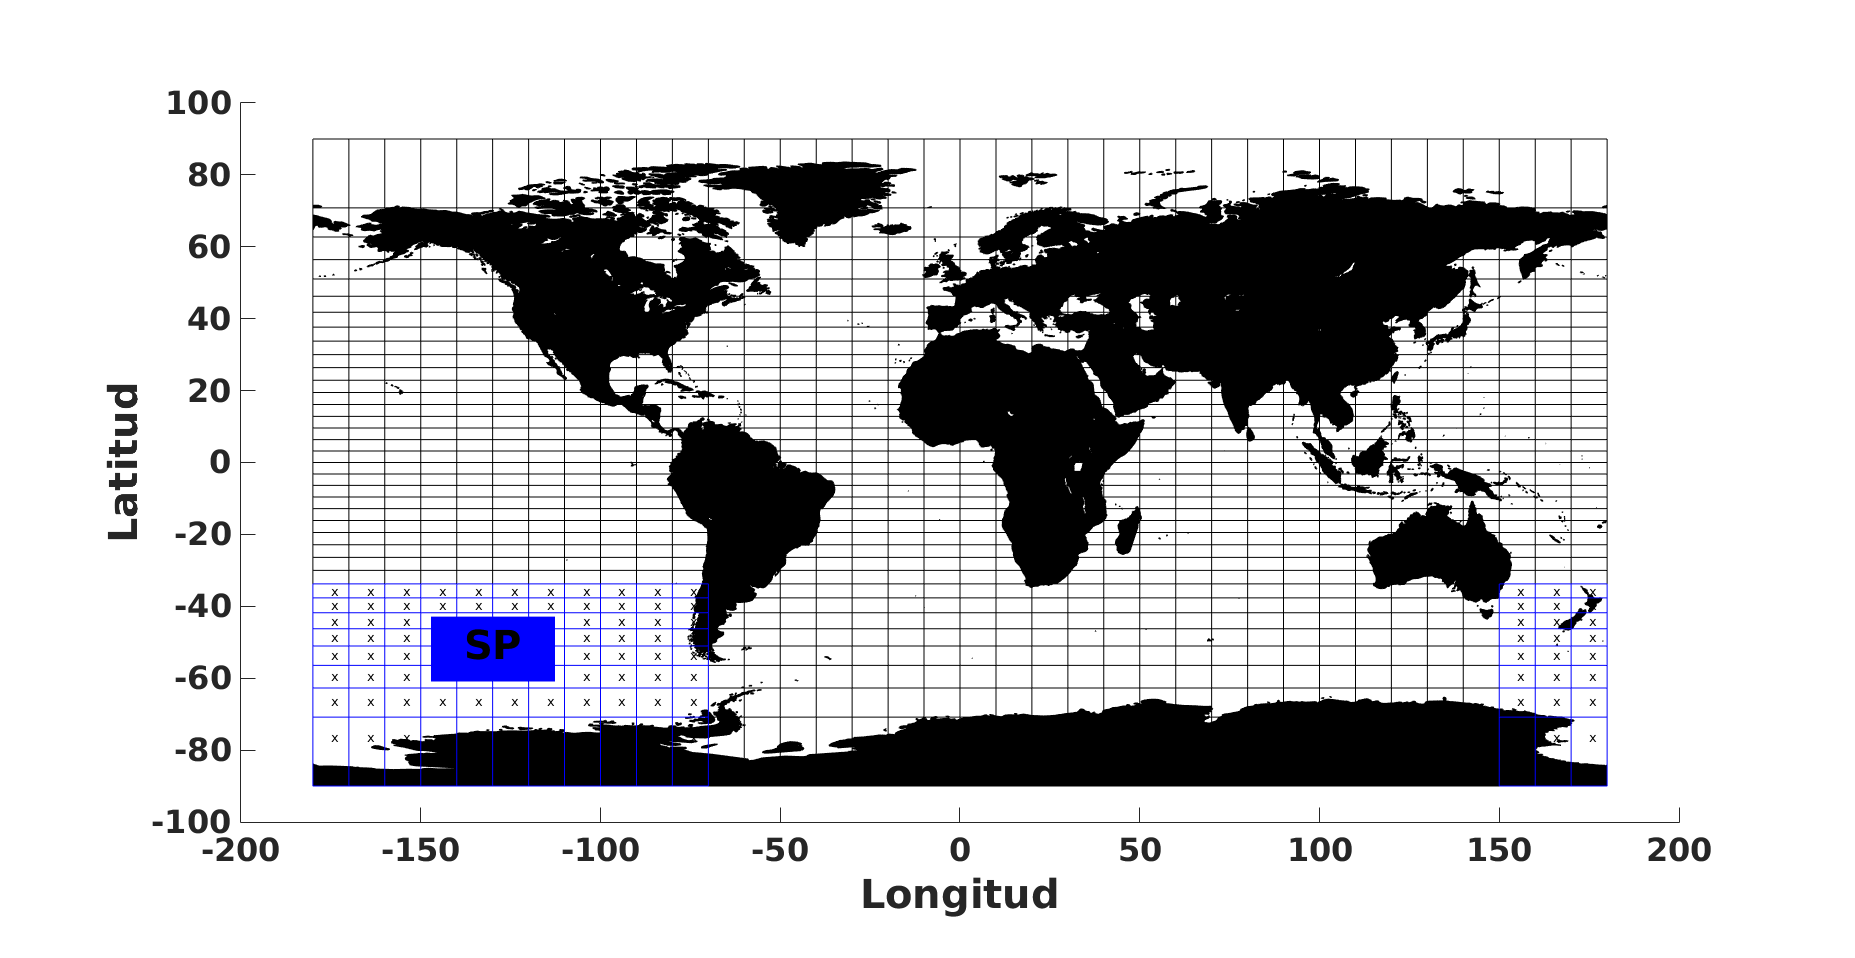
\includegraphics[width=0.8\textwidth]{mapa3_2_SP.png}
 \caption[Figura de región del Pacífico Sur]{Mapa global, que muestra la región del Pacífico Sur que fue aislada en la simulación cGENIE.}
  \label{fig:Mapa_SP}
\end{figure}

\begin{table}[H]
\centering
\begin{tabular}{|c|c|c|c|c|}
\hline
& \multicolumn{4}{c|}{Reducci\'on de $pCO_2$ global} \\
\cline{2-5}
Modelo& Ajuste & Par\'ametros & R-cuadrado ($R^2$) & RMSE\\
\hline \hline
Lambert  & Logar\'itmico  & p1=-22.48, p2=533.5 y p3=3.261 & 1 & 0.0029 \\ \hline
Albani & Logar\'itmico & p1=-457.4, p2=3.241e+04 y p3=63.2 &  0.38 & 0.2088\\ \hline
Takemura & Logar\'itmico & p1=45.27, p2=-816.4 y p3=-8.036 & 0.9982 & 8.0717e-04 \\ \hline
%MIROC-ESM & Lineal & p1=1.23$e^{-13}$ y p2=-1.03 & 0.9942 & 0.06412\\ \hline
%MRI-CGCM3 & Lineal & p1=1.60$e^{-13}$ y p2=-0.99 & 0.9876 & 0.01904\\ \hline
\end{tabular}
\caption[Coeficientes de ajustes SP]{Caracter\'isticas de los ajustes realizados a las reducciones globales de $pCO_2$, a partir de los resultados del modelo cGENIE. El ajuste general es logar\'itmico, 
su ecuaci\'on est\'andar es: $ f(x)=p1 + \frac{p2}{x} + p3*log(x)$. Donde f(x) es la reducci\'on de $pCO_2$ y x, el flujo de polvo de cada nivel para la zona del Pacífico Sur.}
\label{tabla:Res4}
\end{table} \newpage

 \begin{figure}[H]
        \begin{subfigure}[b]{0.5\textwidth}
                \includegraphics[width=\linewidth]{../../Figuras/Regionales/Albani/SP}
                \caption{Albani}
                \label{fig:L_R_SP}
        \end{subfigure}%
        \begin{subfigure}[b]{0.5\textwidth}
                \includegraphics[width=\linewidth]{../../Figuras/Regionales/Lambert/SP}
                \caption{Lambert}
                \label{fig:A_R_SP}
        \end{subfigure}%
        
        \begin{subfigure}[b]{0.5\textwidth}
                \includegraphics[width=\linewidth]{../../Figuras/Regionales/Takemura/SP}
                \caption{Takemura}
                \label{fig:T_R_SP}
        \end{subfigure}%
        \begin{subfigure}[b]{0.5\textwidth}
                \includegraphics[width=\linewidth]{../../Figuras/Regionales/MIROC-ESM/SP}
                \caption{MIROC-ESM}
                \label{fig:MI_R_SP}
        \end{subfigure}
        
        \begin{subfigure}[b]{0.5\textwidth}
                \includegraphics[width=\linewidth]{../../Figuras/Regionales/MRI-CGCM3/SP}
                \caption{MRI-CGCM3}
                \label{fig:MR_R_SP}
        \end{subfigure}
        \caption[Series de reducci\'on de $pCO_2$ de flujos regionales de polvo (SP)]{Reducci\'on de $pCO_2$ obtenidos mediante simulaci\'on cGENIE, para flujos de polvo cambiantes en la zona del Pacífico Sur (SP) desde el Holoceno hasta el \'Ultimo M\'aximo Glacial.}\label{fig:SP}
\end{figure}

El caso Lambert posee los mayores niveles de depositación de polvo en estas latitudes (ver imagen \ref{fig:Mapa_Lambert}). Ésto se refleja en un máximo de reducción de pCO$_2$ de $\sim 4.6$ ppm. No obstante, si bien Albani posee magnitudes de polvo $\sim 5$ veces inferiores en cada nivel comparado con Lambert, tiene una reducción de pCO$_2$ de $\sim 3$ ppm. Ésto, se encuentra asociado a la menor variabilidad de amplitudes UMG:Holoceno (entre $\sim 0.8$ y $1.6$, figura \ref{fig:A}) en comparación a Lambert (entre -0.2 y 1.2) (ver anexo \ref{fig:L}). 

El modelo Takemura, muestra un ínfima reducción de $\sim 0.04$ ppm para el UMG, lo que refleja poco aporte de polvo en estas latitudes (ver \ref{fig:Takemura}). MIROC-ESM y MRI-CGCM3 son modelos que no poseen fuentes de polvo en estas latitudes, por ende, muestra una progresiva disminución de flujo de polvo desde el Holoceno hasta el UMG. El caso más crítico es mostrado por el modelo MIROC-ESM con amplitudes UMG:Holoceno entre -0.4 y 0 (ver Anexo \ref{fig:MI}).   

\subsection{Atl\'antico Sur}

\begin{figure}[H]
\centering
 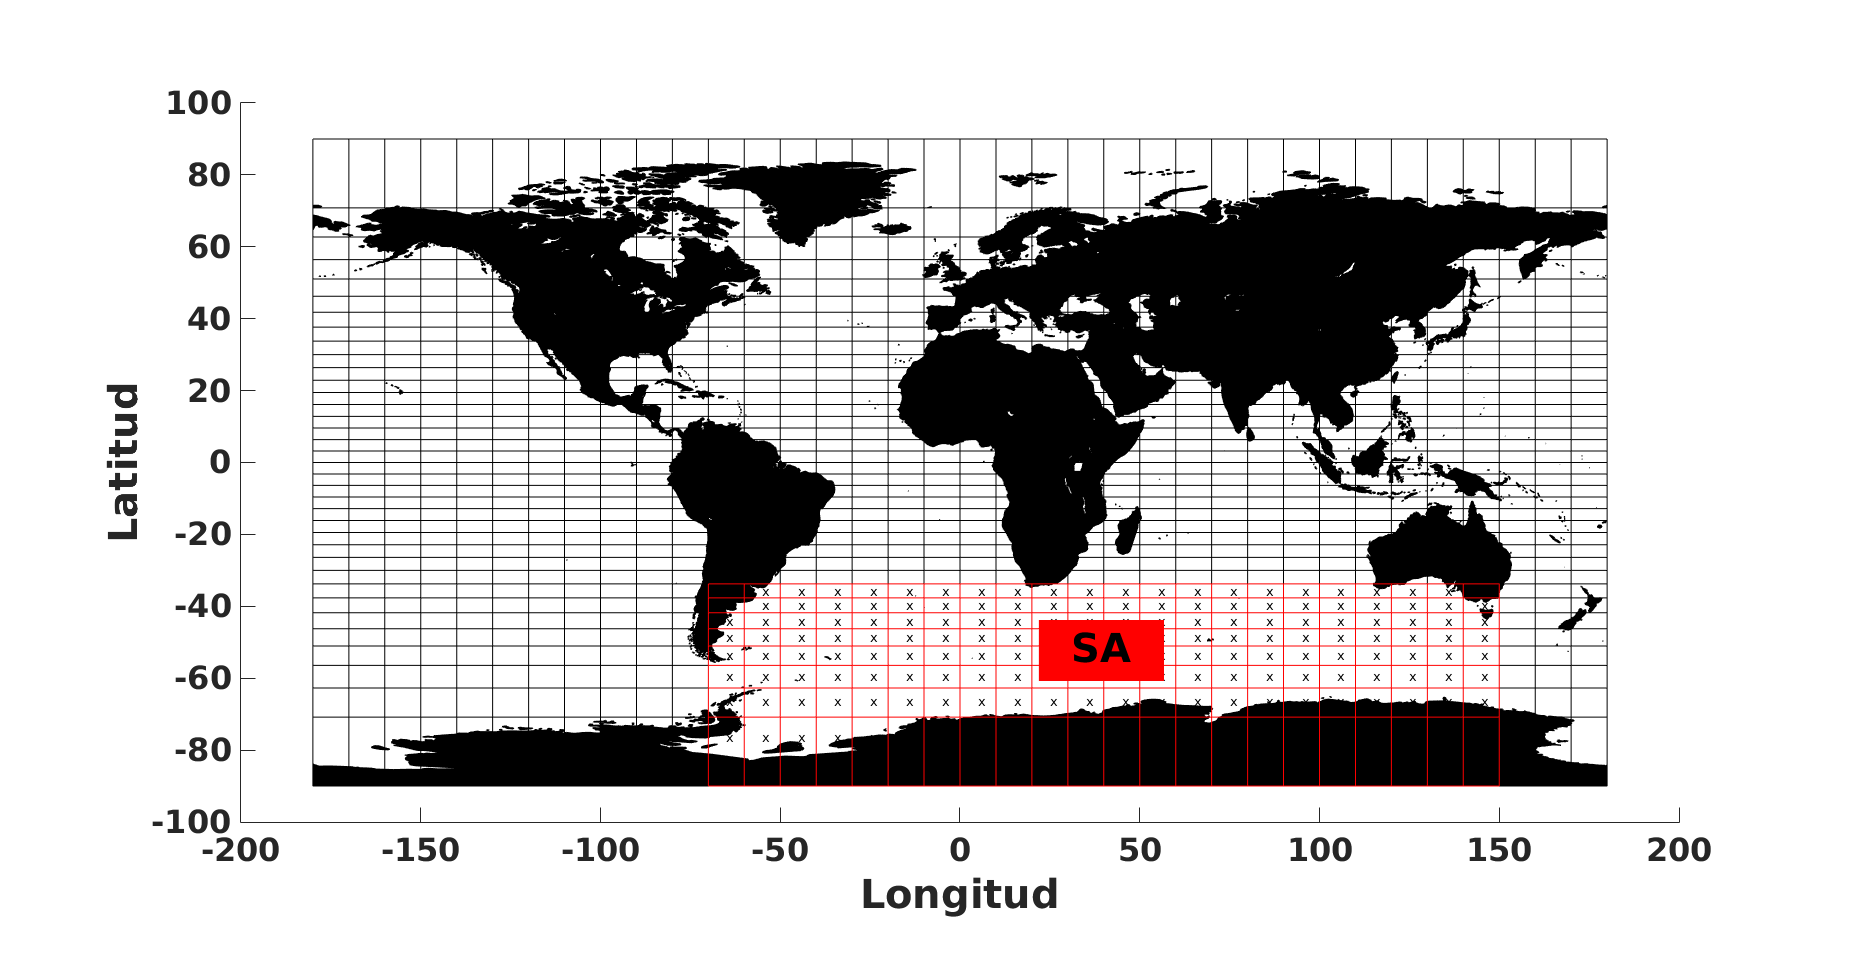
\includegraphics[width=0.8\textwidth]{mapa3_2_SA.png}
 \caption[Figura región del Atlántico Sur]{Mapa global, que muestra la región del Atlántico Sur que fue aislada en la simulación cGENIE.}
  \label{fig:Mapa_SA}
\end{figure}

\begin{table}[H]
\centering
\begin{tabular}{|c|c|c|c|c|}
\hline
& \multicolumn{4}{c|}{Reducci\'on de $pCO_2$ global} \\
\cline{2-5}
Modelo& Ajuste & Par\'ametros & R-cuadrado ($R^2$) & RMSE\\
\hline \hline
Lambert  & Logar\'itmico  & p1=-69.08, p2=1.47e+04 y p3=8.09 & 0.9986 & 0.0808 \\ \hline
Albani & Logar\'itmico & p1=-18.92, p2=-72.4 y p3=3.116 & 0.9993 & 0.1232\\ \hline
%Takemura & Lineal & p1=1.14$e^{-13}$ y p2=-1.3 & 0.9966 & 0.03623\\ \hline
%MIROC-ESM & Lineal & p1=1.23$e^{-13}$ y p2=-1.03 & 0.9942 & 0.06412\\ \hline
MRI-CGCM3 & Logar\'itmico & p1=-26.43, p2=1258 y p3=3.492 & 0.9999 & 0.01040\\ \hline
\end{tabular}
\caption[Coeficientes ajuste SA]{Caracter\'isticas de los ajustes realizados a las reducciones globales de $pCO_2$, a partir de los resultados del modelo cGENIE. El ajuste general es logar\'itmico, 
su ecuaci\'on est\'andar es: $ f(x)=p1 + \frac{p2}{x} + p3*log(x)$. Donde f(x) es la reducci\'on de $pCO_2$ y x, el flujo de polvo de cada nivel para la zona del Atlántico sur. }
\label{tabla:Res5}
\end{table}

 \begin{figure}[H]
        \begin{subfigure}[b]{0.5\textwidth}
                \includegraphics[width=\linewidth]{../../Figuras/Regionales/Albani/SA}
                \caption{Albani}
                \label{fig:L_R_SA}
        \end{subfigure}%
        \begin{subfigure}[b]{0.5\textwidth}
                \includegraphics[width=\linewidth]{../../Figuras/Regionales/Lambert/SA_log}
                \caption{Lambert}
                \label{fig:A_R_SA}
        \end{subfigure}%
        
        \begin{subfigure}[b]{0.5\textwidth}
                \includegraphics[width=\linewidth]{../../Figuras/Regionales/Takemura/SA}
                \caption{Takemura}
                \label{fig:T_R_SA}
        \end{subfigure}%
        \begin{subfigure}[b]{0.5\textwidth}
                \includegraphics[width=\linewidth]{../../Figuras/Regionales/MIROC-ESM/SA}
                \caption{MIROC-ESM}
                \label{fig:MI_R_SA}
        \end{subfigure}
        
        \begin{subfigure}[b]{0.5\textwidth}
                \includegraphics[width=\linewidth]{../../Figuras/Regionales/MRI-CGCM3/SA}
                \caption{MRI-CGCM3}
                \label{fig:MR_R_SA}
        \end{subfigure}
        \caption[Series de reducci\'on de $pCO_2$ de flujos regionales de polvo (SA)]{Reducci\'on de $pCO_2$ obtenidos mediante simulaci\'on cGENIE, para flujos de polvo cambiantes en la zona del Atlántico Sur (SA) desde el Holoceno hasta el \'Ultimo M\'aximo Glacial.}\label{fig:SA}
\end{figure}

La simulación de Albani, tiene la mayor reducción de pCO$_2$ estimada para el UMG ($\sim 12.5$ ppm). La figura \ref{fig:Albani}, muestra la existencia de una intensa fuente de polvo localizada en América del Sur, en las cercanías de la Patagonia chileno-argentina. Esto explica las altas tasas de depositación de polvo en relación a los otros casos (la amplitud UMG:Holoceno alcanza valores entre 1.2-1.4). 

La reconstrucción Lambert con también una fuente de polvo en la zona Pagónica de Sur América, aunque con valores inferiores a los estimados por Albani, y con más estrechas diferencias entre el Holoceno y UMG, tienen una disminución de pCO$_2$ de $\sim 6$ ppm. A su vez, MRI-CGCM3 posee una muy pequeña fuente de polvo en la misma zona (ver figura \ref{fig:MRI}), lo que se traduce en que los flujos de polvo produzcan una disminución de pCO$_2$ de $\sim 1$ ppm. En relación a Takemura y MIROC-ESM, ambos no poseen fuentes de polvo en la zona cercana al Atlántico Sur, por ende, en ambos casos el modelo cGENIE simula una progresiva liberación de CO$_2$ desde el océano hacia la atmósfera, alcanzado valores de -0.49 y -1.22 ppm desde el Holoceno al UMG respectivamente. 


\section{Resultados finales}

\begin{figure}[H]
\centering
 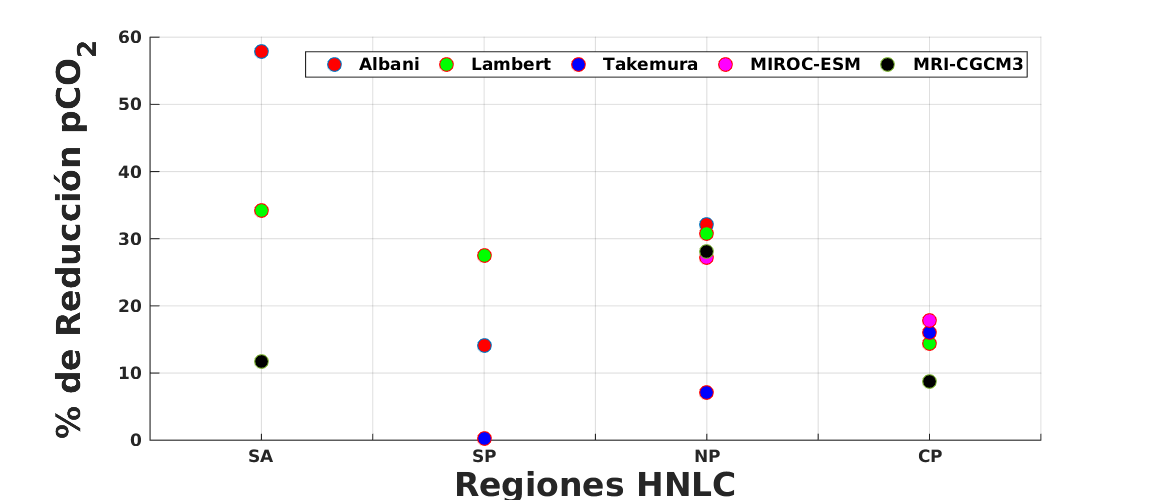
\includegraphics[width=0.85\textwidth]{../../Figuras/Ponderaciones/Ponderaciones_LGM}
 \caption[Contribución ponderada de las zonas HNLC a la reducción de CO$_2$ global]{Contribución ponderada de las zonas HNLC (Atlántico Sur, Pacífico Sur, Pacífico Norte y Pacífico Central) a la reducción de pCO$_2$ global. En rojo las contribución relativa del modelo Albani, en verde la correspondiente a la reconstrucción Lambert, en morado la contribución Takemura, en rosado el aporte de MIROC-ESM y en negro la participación de MRI-CGCM3.   }
  \label{fig:Ponderacion}
\end{figure}

En la figura \ref{fig:Ponderacion} sólo se consideraron las simulaciones que reflejaban un incremento en los campos de polvo y, por lo tanto, un progresivo aumento en la captación de pCO$_2$ por parte de las distintas regiones oceánicas (SA, SP, NP, CP), en relación a su reducción total. 

En concordancia con los resultados regionales, vemos que las respuesta de los distintos casos y sus respectivos flujos de polvo en la región CP, tiene un menor aporte a la reducción total en cualquiera de las simulaciones. Sin embargo, vemos también que los campos de polvo en esta latitud son menores en relación a otras zonas en todos los casos (ver figuras del UMG en el capítulo 4 y \ref{fig:MR}). Además que la zona muestra en general un gradiente zonal de depositación, con mayores flujos en la zona este del Pacifico y menor en la zona oeste. No obstante, esta región presenta un buen ajuste de las simulaciones quedando rezagado sólo el modelo MRI-CGCM3, el cual como vimos es el que menor captación tiene en el área ($\sim 0.8$ ppm) para un total de $\sim 9$ ppm producto de la mínima presencia de flujo de polvo registrada por el modelo en cada nivel del periodo de estudio (ver figura \ref{fig:MRI}). Así la media de reducción de pCO$_2$ calculada entre las distintas simulaciones se encuentra en torno a los 2.4 ppm, es decir, un $\sim 15\%$ de aporte en la captura de esta región oceánica. 


La región del Pacífico Norte, muestra un buen acuerdo entre los modelos en torno a la mayor participación de la región en la reducción de pCO$_2$ global ($\sim 30\% $), a pesar de la alta variabilidad en los flujos de polvo. La zona NP tiene una media de $\sim 5$ ppm. Lo que implica que los modelos de polvo presentan un intrusión importante de flujo en el área, cuya sensibilidad producto de la depositación es alta y se ve reflejado en la biogeoquímica de la productividad biológica establecida en cGENIE. El modelo Takemura, no presenta fuente de polvo en las cercanías de esta zona (ver figura \ref{fig:Takemura}). 

Por otro lado, la región SP con una media de $\sim 1.55$ ppm, representa una contribución del $\sim 14\%$. Sin embargo, vemos que la variabilidad de las reducciones entre los distintos casos depende de la intensidad y de la ubicación de la fuente de polvo para esta zona. Dado que los modelos muestra grandes diferencias en los flujos de polvo, no se puede asegurar el porcentaje de participación en la captura de pCO$_2$, pero si se puede afirmar que en presencia de una fuente de polvo, esta zona oceánica responderá en su biología al eventual suministro de hierro. 

La región SA muestra ser la que más aporta en la captura de pCO$_2$, rangeando entre $\sim 11\%$ para valores bajos de suministro de polvo y $\sim 58\%$ para suministro mayores (con una media de $\sim 34\%$). Si bien, no hay un buen ajuste entre los modelos en torno a la cantidad de polvo en los distintos niveles y en particular para el UMG, si se ve que existe una alta sensibilidad a la magnitud del suministro en esta región oceánica, y que será la que mayor captura realice (Lambert tiene el doble de flujo de polvo en NP que en SA, sus capturas respectivamente son $\sim 5$ p.p.m. y $\sim 6$ ppm). 

Finalmente, vemos que la reconstrucción Lambert, posee una buena asimilación por parte del modelo cGENIE en todas las simulaciones, además que guarda cierta prudencia en cada una de sus estimaciones. No obstante, posee una gran variabilidad que no es capturada por otros modelos de flujos de polvo vistos en este trabajo. Por ende, se requieren mayores comparaciones para darle un mayor grado de confianza. Por otro lado, el modelo MIROC-ESM es el que muestra menos presencia en las simulaciones, debido su escasa existencia de fuentes en el Hemisferio Sur, además parece tener una drástica respuesta en sus estimaciones para distintas zonas, por ende, parece ser el modelo más débil en esta investigación. Los campos de polvo MRI-CGCM3 han resultado hasta ahora, las simulaciones más reservadas de captura de pCO$_2$. 